\section{Network Implementation Concerns}
Separating content networks from physical networks enables network infrastructure virtualization and multi-tenancy.  Use the popular file-sharing system BitTorrent as an example.  BitTorrent is a content network optimized for download efficiency.  It run over traditional TCP/IP networks, but manages traffic according to specialized algorithms unique to BitTorrent.  These algorithms take advantage of the asymmetry between upload and download speeds of typical home-use Internet systems in which upload speeds are regularly an order of magnitude slower than download speeds.  By partitioning content into distinct sections and downloading them from multiple clients, a downloading node can effectively use all available download bandwidth and is no longer necessarily constrained by the upload bandwidth of a serving peer system.  These systems use a similar approach, in that these hypothesized systems also overlay TCP/IP traffic, but rather than optimizing download speeds they focus on content usage management.

Just as systems like BitTorrent runs over current established protocols, usage management overlay systems could as well.  They support multi-tenant cloud computing systems by providing secure compartmentalized access to managed information.  They also support the ability to create and use integrated overlay systems between multiple cloud providers, supporting running of overlay components in systems hosted at Amazon while accessing nodes executing on Rackspace infrastructure.

Content networks must deal with situations analogous to those encountered in previous physical systems.  Specific examples include cross-domain monitoring and content mashing.  Both problems are currently areas of active research within physical networks and need extensive examination in overlay systems as well.

To begin with, in content-specific overlay networks, cross-domain routing can become an even more pervasive issue.  Currently, cross-domain data processing guards are installed on the perimeter of sensitive networks where they can monitor and manage outgoing and incoming traffic.  In content networks, these kinds of systems can begin to multiply within the information transmission fabric.  In physical networks, the network topology is fixed and is established when the network is installed.  After installation, changes in the essential network topology are cost-prohibitive and correspondingly rare.  Overlay systems do not suffer from this high cost of change, and can easily morph from one topology to another.  As additional content enclaves appear within a given overlay topology, the need for content usage management between those enclaves increases.

Mashup scenarios become similarly common.  As additional sources of accessible data appear, opportunities for inappropriate data combinations increase at best geometrically.  Data combinations need to be likewise managed to prevent inappropriate data combinations.

\section{Initial Prototype Implementation}
Our first completed prototype shows that overlay routers can in fact use licenses bundled alongside content to modify transmitted content based on dynamic network conditions.  Running on a single host over HTTP, it simulates two content domains and communication between them.  The communication link has uncertain security state and changes over time.  Note that this prototype currently runs on a single host with varying ports, but it could easily run on multiple hosts as well.  The current single host configuration is simply to simplify system startup and shutdown.

\begin{figure*}[!t]
\centering
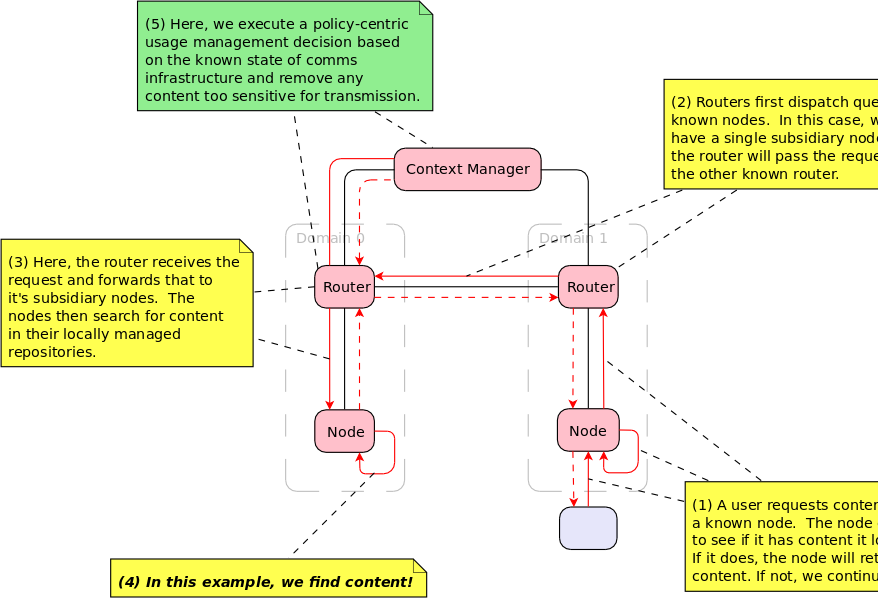
\includegraphics[width=6in]{cross-domain-prototype}
\caption{Simulation Logical Configuration}
\label{fig:model:cross-domain-prototype}
\end{figure*}

License bundles are hosted on the filesystem, though they could be hosted in any other data store.  These artifacts are currently XML.  They are stored in a directory, and the license file has a LIC extention while the content file has an XML extension.  Both the content and the license files have the name of the directory in which they reside (for example, if the directory is named test, the license file is named test.lic and the content file test.xml).  In this context, the directory is the content bundle.  The license and content files are simply documents and port to document-centric storage systems like MongoDB easily.  They can certainly be stored in traditional relational databases as well.

The system itself has two domains, Domain 0 and Domain 1.  Each domain consists of a client node and a content router node.  Requests are initially served to client nodes.  If client nodes do not contain the requested content, they the forward that request to their affiliated content router.  The content router will send that request to all the content routers of which it is aware.  Those other routers will then query associated client nodes for content.  If the requested content is in fact found, it will be returned to the original requesting router and then to the requesting node.  If the content is not found, HTTP status 404 codes are returned to requesting routers and nodes.

All router-to-router content traffic is modified based on security conditions.  A Context Manager maintains metadata regarding network paths.  If a given network path is only cleared for data of a certain sensitivity level, a transmitting router will remove all license information and content that is associated with higher sensitivities, and then transmit only information at an appropriate sensitivity level over the link.

Figure \ref{fig:model:cross-domain-prototype} shows the prototypical workflow through the system across the domains, and Figure \ref{fig:model:prototype-physical-config} shows the current system configuration of the simulation, with the cross-domain link highlighted in red.  The system is current configured to use ports 4567 through 4571.

All content requests are via HTTP GET.  Link status can be changed via HTTP POST and the CURL command is used to access the network.

This proof-of-concept does implement a simple overlay network for usage managed content over HTTP, easily extensible to HTTPS.  Changes in the context of the network dynamically change the format of transmitted content.  All source code for this simulation is publically available on GitHub, at https://github.com/cclamb/overlay-network, with documentation on how to run the simulation.

\begin{figure}[!t]
\centering
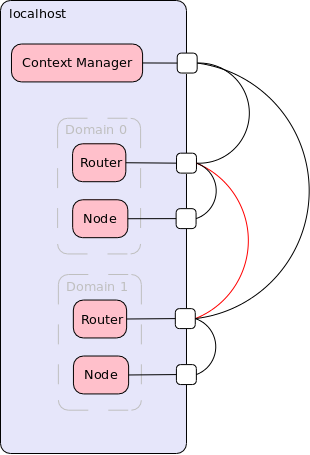
\includegraphics[width=3in]{prototype-physical-config}
\caption{Physical Simulation Configuration}
\label{fig:model:prototype-physical-config}
\end{figure}

Initial results confirmed that the approach was feasible.  The network was able to successfully filter content based on policies and dynamic network conditions.  The system was also able to deliver both arbitrary content and policies within a single document as well, and it was not prohibitively difficult to extract either data or policies.  Furthermore, Ruby with Sinatra effectively supported the required HTTP-centric infrastructure needed to effectively simulate an information-centric network.  It seemed clear at this point that extending the prototypical implementation from a single host to a fully nationally distributed network was feasible.

\section{Inter-Provider Cloud Configuration}
At this point, I have created and deployed baseline system images in both Amazon's Elastic Compute Cloud (EC2) and Rackspace Servers infrastructures.  I have also created and exercised our deployment, configuration, and logging systems to enable distributed monitoring and centralized reporting.  Overall, the system currently has 20 nodes running with two distinct providers geographically dispersed across the continental United States.  This leads to a distinct requirement for a centralized system with distributed access for both initial configuration information as well as logging and auditing.  This required infrastructure has been implemented using Amazon's Simple Storage Service (S3), accessible from both Rackspace and Amazon hosted virtual machines.

The specific technical components are Amazon EC2, Amazon S2, Rackspace Servers, and GitHub.  Both EC2 and Rackspace nodes are Ubuntu virtual machines, albeit at different versions, specifically Ubuntu version 11.04 in Rackspace and Ubuntu Version 12.04 in Amazon's infrastructures.  These systems are provisioned with Git, Ruby, the Ruby Version Manager (RVM), and supporting libraries.  They all run as micro-intances or equivalent, and are bootstrapped with the appopriate project information to begin to participate as an overlay network node.  While EC2 and Rackspace Server infrastructures are infrastructure-as-a-cloud (IaaS) offerings supporting virtual machine instances of various types, Amazon S3 is a simple key-value store.  Running with REST sematics over HTTP, S3 stores arbitrary documents associated with specific keys in buckets.  These documents can be downloaded by any authorized participant, where authoriztion state is proven by possention of a secret key.  In this way, the global configuration of a specific overlay network can be stored in a single location from which every node can access informationm with respect to their pending role and needed configuraiton information.  Likewise, all overlay network state can also be saved to centralized buckets for later analysis.  Finally, Github is a centralized source code repository used to share code between all participating nodes.  Prior to each content network instantiation, each node checks the repository for updates, and downloads them if they exist.

\begin{table*}[tp] %
\centering %
\begin{tabular}{lc}
\toprule %
$Category$ 				& $Components$ 								\\\toprule %
$Infrastructure$ 		& Amazon S3, Amazon EC2, Rackspace Servers 	\\\midrule
$Operating Systems$		& Ubuntu 11.04, Ubuntu 12.04 				\\\midrule
$Technologies$			& Ruby (Sinatra, Capistrano, YAML) 			\\\midrule
$Supporting Systems$		& Git, Github 								\\\bottomrule
\end{tabular}
\caption{Supporting Components}
\label{table:model:components}
\end{table*}

All data saved within S3 is serialized in a text-based data serialization language known as YAML.  YAML is a widely supported hierarchical data representation language with support within the Ruby core platform.  This enables us easily serialize Ruby-native data structures to text-based representations for storage within S3.  More importantly, it simplifies post-experimental data analysis as any information logged to the centralized logging system during a given experimental run can be easily read and analyzed after the fact.

Capistrano is used in order to manage and initialize all overlay nodes.  Capistrano is a distributed deployment system initially used to manage large clusters of Ruby-on-Rails systems.  It has since expanded into a general-purpose distributed deployment toolchain, tightly integratd with Git.  This allows us to bootstrap different configurations of networks from a single command-and-control node simply and efficiently.

\section{Inter-Cloud Architecture}
At this point the system is a distributed content network distributed across multiple nodes and domains providing cross-domain managed data access.  This network consists of clients accessing information through a user interface subsystem that accesses data from external sources and a distributed cross-domain information network.  Queries are submitted through a client, to an application server, then to external services and information nodes.

The unique strength of this system is enabling dynamic distributed content control.  This includes information retraction, redaction, protection, and secure routing.  Information retraction involves quickly removing a user's access to sensitive data.  Redaction addresses simple data removal, while protection would operationally involve applying encryption layers of increasing strength based on operational demands.  Finally, secure routing would provide the ability to send data over a more secure link if such a link is available and required.

In this system information retraction involves changing the execution context such that access for a given user, perhaps even on a specific device, is removed.  This context then propagates through the information network and attached clients.  This is useful when a given user, say a coalition partner, is suddenly considered compromised and can no longer be allowed access to sensitive information.  Likewise, a specific user's system may likewise be compromised and be forbidden access to specific information.

Information redaction is generally used when a user simply does not have authorization for a specific section of content, generally within a larger document. In these cases, that information and related policy metadata are simply removed from any query responses.  Likewise, information protection also addresses specific subsections of information in a larger document, but unlike redaction, a user is in these cases authorized to access information, but one of the links over which the information must travel is not authorized to transmit specific sensitive information.  In these cases that information can be encrypted with appropriately strong encryption to allow for more secure information transmission.

Finally, secure routing use directly addresses the ability to select communication links based on information content.  In these situations, a network has more than one path over which to return content.  Furthermore, these multiple paths have different characteristics providing different levels of service.  The system, based on rules contained in a policy and the current context can then select communication links of different security levels when returning content.Likewise, the content network must:

\begin{itemize}
\item Support and distribute queries for available content based on submitted constraints including artifact key and hop count.
\item Support and distribute queries for specific content based on key.
\item Evaluate returned content for suitability for transmission to a requesting node at each transmission step.
\item Support partitioning into multiple domains.
\item Allow for dynamic information distribution at network start.
\item Collect experimental metrics for evaluation.
\item Be distributed across multiple nodes.
\end{itemize}

Overall, the system consists of an HTML 5 based user interface subsystem, external data sources, and a content network, as shown in Figure 1.  The user interface layer displays maps and associated metadata to users based on submitted geolocation information and supports two different mobile profiles (tablet and telephone) and a single workstation profile.  HTML 5 media queries were used for end device detection, allowing us to format information differently for our three profiles facilitating usability.  External data sources could be any data programming interface offered by a third party.  In this system, Google Maps was used to define, download, display, and format maps.  Finally, this content network exists and is configurable either as a hierarchical network or a non-hierarchical network containing geo-tagged information at various sensitivity levels.  This content network can be configured arbitrarily, enabling the creation of a virtually unlimited number of different information domains.

\begin{figure}[!t]
\centering
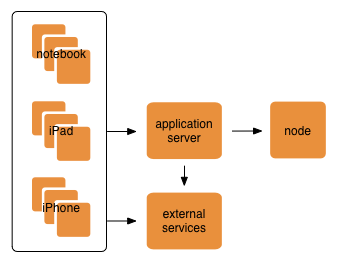
\includegraphics[width=4in]{overall-view}
\caption{Overall System Architecture}
\label{fig:model:overall-view}
\end{figure}

In this work, the client systems layer will be replaced with a command-line interface and external services will not be accessed, but a typical deployment operationally would have these elements.

The user interface subsystem processes requests and returns information from both Google Maps and the content network based on those requests.  Technically, it is based on the latest version of Ruby on Rails (RoR) using standard RoR configuration conventions running on top of Ruby 1.9.*.  Rake is used for deployment, and Gem for component installation.  Bundler is used to maintain consistent application dependency state and RVM to manage Ruby virtual machine versions.  HTML 5 interface elements are defined using SASS and HAML.

Operationally, typical system use involves query submission, usage management rectification,  and result display.  Two distinct types of queries exist - an initial query for a map of a specific location, generally triggered by entering some kind of geolocation parameters (though potentially using device-generated location information, allowing automatic map alignment with a user's current location) and a query for specific sensitive information.  Initial queries have two distinct subqueries, one of map information directed at the Google Maps API, and another of the content network to see what data is available.  All content is usage managed to ensure that mashed information is consistent from a data sensitivity perspective prior to display to the user.  Currently, no information is cached within the interface subsystem.

\begin{figure}[!t]
\centering
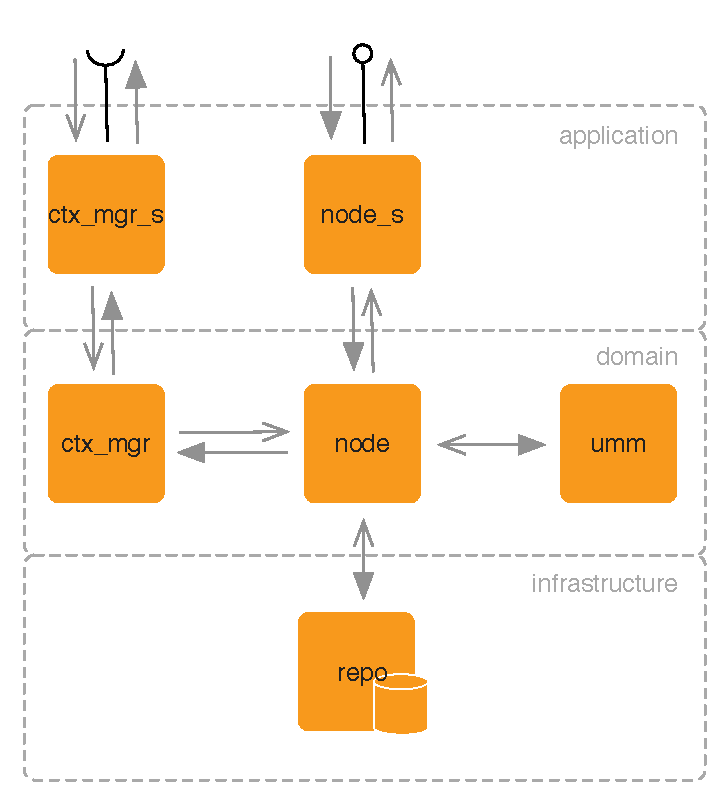
\includegraphics[width=4in]{node-view}
\caption{Node Architecture}
\label{fig:model:node-view}
\end{figure}

The content network can be configured to run as an HTTP overlay system using HTTP routers and nodes or in a peer-to-peer configuration.  In either case, queries can be submitted to the network from any one of the constituent nodes - note that routers do not store data; rather, they focus soley on routing queries through a hierarchical network.  After initial submission, queries propagate throughout the network based on user-submitted search parameters.  The content network physically runs on nodes provisioned from Rackspace Cloud and Amazon Elastic Compute Cloud (EC2).  It is built using Sinatra for HTTP processing and uses Capistrano for distributed system deployment and control.  Distributed data is stored in Amazon Simple Storage Service (S3) buckets.  RVM, Gem, and Bundler are used in this system as in the user interface subsystem.

In both configurations, the common functional flow is built around responding to content queries with information of appropriate sensitivity for a given query context, as shown in Figures \ref{fig:model:node-view} and \ref{fig:model:router-view}.  In general, systems are designed with a layered perspective, with an application layer fielding initial requests, a protocol-agnostic domain layer that manages query responses, and an infrastructure layer that contains specific required libraries and other technical artifacts.  In these systems, the application layer handles HTTP protocol issues, translating requests from the lingua franca of HTTP into the domain language reflected in the domain layer.  The infrastructure layer consists of various data management technologies called upon by the domain layer when needed.

Figures \ref{fig:model:node-view} and \ref{fig:model:router-view} highlights communication ordering within components in a hierarchical content network and also shows the functional components within the system.  From a communication perspective, requests come in through the application layer and are then handed off for processing to the domain layer.  The domain layer retrieves the current context and is responsible for query dispatch (in the case of a router) or data reponses (in the case of a node) that are managed according to the current environmental context.

\begin{figure}[!t]
\centering
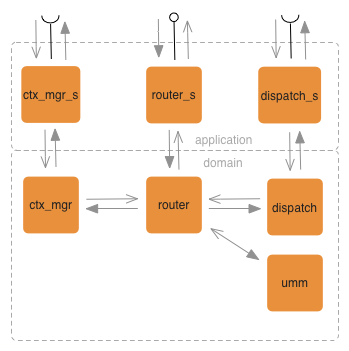
\includegraphics[width=4in]{router-view}
\caption{Router Architecture}
\label{fig:model:router-view}
\end{figure}

The primary components in the router and node systems' application layer are small adapters intended to translate between HTTP protocols and domain components.  They are:

\begin{itemize}
\item \textbf{Context Manager Client Service (ctx\_mgr\_s)} --- This is an adapter between the domain context manager and the external context service.
\item \textbf{Node Service (node\_s)} --- The node service provides a RESTful interface to external clients.  All content requests are initially sent to a known node service.  This is essentially the external interface to a given content network.  A content network generally contains many distinct nodes as well.
\item \textbf{Router Service (router\_s)} --- The router service is essentially a customized HTTP router that dispatches content requests and responses through a hierarchical content network in accordance with established policies and the current environmental context.
\item \textbf{Dispatch Service (dispatch\_s)} --- This service dispatches information requests to known nodes based on known policies and context.
\end{itemize}

The domain layer components include:

\begin{itemize}
\item \textbf{Context Manager (ctx\_mgr)} --- The context manager client service calls into the context manager service to retrieve the most current contextual information with respect to the content network, attached clients, users, and devices.
\item \textbf{Node (node)} --- The node component contains all logic needed to process and respond to information requests.  Nodes manage requests, responses, context evaluation, and usage management mechanism application.
\item \textbf{Usage Management Mechanism (umm)} --- The usage management mechanism will apply rules grouped into policies against a known context to determine the acceptability of an intended action.  It will indicate whether or not that action can proceed.  It can also make changes to a proposed action so that the alternative action can be executed.
\item \textbf{Router (router)} --- Router domain components manage the distribution of information requests and responses, applying managing information dispersal throughout a content network in accordance with context and policy.
\item \textbf{Dispatcher (dispatch)} --- Dispatchers send requests to known routers or nodes in the larger context network.
\end{itemize}

Finally, the sole infrastructure component:

\begin{itemize}
\item \textbf{Information and Policy Repository (repo)} --- Unique to nodes, information and policy repositories contain specific network content, organized by key, and associated policies.
\end{itemize}

The same components are used to assemble non-hierarchical networks, in which nodes have both content and policy storage as well as request response and dispatching responsibilities.  Also note that context management and usage management components are shared between all types of content networks as well as all types of component systems within those networks.  Non-hierarchical nodes and hierarchical routers and nodes all need these kinds of services.

\section{Experimental Structure}
Content-centric networks are generalized constructs supplying the ability to manage distributed content more effectively.  This work explores specifically how users can control information security and privacy in a more granular way when data is arbitrarily combined.  In order to do this effectively however, a simple protocol must be defined that allows connected systems to determine what kind of information is available.

A variety of approaches can be used with respect to information storage in these kinds of networks.  In many ways, they exhibit behavior very similar to filesystems.  In a content-centric network, rather than asking for content via some kind of address, like a uniform resource locator (URL), a specific non-ambiguous name is used.  This is very similar to how content management systems and web caches work today.  These kinds of systems treat a URL as a name rather than an address, returning a cached image of the requested content rather than the content actually pointed to by the URL.  This requires that consumers and caching agents recognize and manage the possibility of stale data, but that risk is generally worth the performance gain.  Content-centric networks can similarly optimize various aspects of content retrieval, returning the most local, highest quality, or most reliable data item, for example.

In this content network, metadata is associated with specific locations as well as the locations themselves.  Rather than optimizing with regard to location or quality, this network optimizes security posture.  In order to do so, a simple data discovery protocol is in place so clients can discover what data is available.

Two different models support content access in this kind of network.  The first, the Cat Model, mimics typical filesystem interaction on unix-centric computers.  The second, the Index Model, acts more like a typical website, with a central index providing available options.  Both models are can manage hierarchical content, a requirement for managing large volumes of information.

The first system is modeled after a typical filesystem.  In this case, a user would have read access to the network via a set of related commands.  Filesystems follow a model where you can list the available contents, access specific details of the contents, and then access individual contents themselves.  In UNIX and unix inspired systems, these actions correspond to ls, for diretory listings, and programs like cat, to allow access to specific individual content.  File details are exposed by options on the ls command.

Command-line access to a content network is certainly feasible.  Command-line shells are common in a variety of environments, ranging from development environments like Play to software development systems like Ruby and Python.

In our content network, the ls command would traverse the network returning information describing contents based on the current security context.  This context consists of the environment, the resource requested, and the subject requesting the resource.  For example, a user with access to a content network via some kind of shell may list network content from a device at a given physical and network location and receive content listing A, while executing a listing from a different device from the same locations may generate content listing B, which can be significantly different from A based on contextual changes.

Another problem arises with listing network contents is the fundamentally different nature of listing a relatively small directory on a local computer as opposed to the contents of a geographically dispersed network.  The latency involved when reading this kind of local directory is small, and the number of elements to list is tractable.  Networks do not support these kinds of assumptions.  The time required to list the available contents on a dispersed content network can be significant.

A cat-like command on a content network suffers from similar problems.  As content within an artifact can be marked with different sensitivity, displayed artifact content can change based on context as well.  Likewise, large artifacts can take significant time to display on devices because of content dispersion issues.

The proposed Index Model has significant precedent as well.  This model is commonly used in world-wide-web systems both large and small.  Modified versions have been used to seed BitTorrent networks as well as direct content traffic on early instances of Napster.  Here, we have a small index file that lists available content on the network.  This index could be associated with a policy and marked for sensitivity, and could contain links to content as well as metadata describing that content.  This index would essentially serve the function of the ls command in the Cat Model.  Selecting a link from an index via a network client would then serve as the Cat Model's cat command.

Similar issues with respect to network dispersion exist with showing the contents of artifacts in both models, and the index contents can seem to change with respect to changing context, as they are also associated with policy sets describing the use of content.  Both models can also be optimized for project-centric content viewing or to show indicators with respect to expected content retrieval latency.  Organizationally, any kind of informational hierarchy within the network would need to be based on the semantics of referenced content rather than external factors.  Content-centric networks use keys to location content rather than addresses, so this hierarchical name would in fact be such a key rather than an address for the content.

Latency effects and content surprise are characteristics of the underlying content network rather than a specific interface approach.  They effect either approach equally.  The Cat Model is more general than the Index Model however.  You can in fact implement the Index Model with the Cat Model, but not the inverse.  Our work is focused on secure mashing of content in a web-centric environment.  As a result, the Index Model fits our needs better than the more general Cat Model.

\subsection{Initial Seed Information}
In order to seed network clients, we provide an initial index object that contains location information and associated metadata.  This information is classed according to sensitivity and consists of names and latitude/longitude coordinates contained in an XML file, similar to that shown in listing \ref{lst:seed-data}.

\begin{lstlisting}[language=xml, label=lst:seed-data, caption=Seed Information for the Network]
<index>
  <location>
    <name>The location name; a city name, for example</name>
    <lat>The location latitude</lat>
    <lon>The location longitude</lon>
    <about>Metadata about the location</about>
    <key>The detail data object name</key>
    <key>...</key>
    ....
  </location>
  <location>...</location>
  <location>...</location>
  ...
</index>
\end{lstlisting}

Any of these XML elements can be marked with an attribute, policy-set, which is the name of a policy set contained in the associated policy file.  It is contained as an artifact with an associated policy set.

Detail data objects are arbitrary XML documents that support the policy attribute.  We support text, images, and shape information.  Each different type is ensconced within an XML element corresponding to the type of data contained, and are delivered in a single XML document with associated policy sets.


\par\noindent
\begin{minipage}[t]{.30\textwidth}
\begin{lstlisting}[language=xml, label=lst:image-data, caption=Image]
<artifact>
  <policy-set>
  ...
  </policy-set>
  <data-object>
    <image type=".">
    ...
    </image>
  </data-object>
  ...
</artifact>
\end{lstlisting}
\end{minipage}
\hfill
\begin{minipage}[t]{.30\textwidth}
\begin{lstlisting}[language=xml, label=lst:shape-data, caption=Shape]
<artifact>
  <policy-set>
  ...
  </policy-set>
  <data-object>
    <shape type=".">
    ...
    </shape>
  </data-object>
  ...
</artifact>
\end{lstlisting}
\end{minipage}
\hfill
\begin{minipage}[t]{.30\textwidth}
\begin{lstlisting}[language=xml, label=lst:content-data, caption=Content]
<artifact>
  <policy-set>
  ...
  </policy-set>
  <data-object>
    <content type=".">
     ...
    </content>
  </data-object>
  ...
</artifact>
\end{lstlisting}
\end{minipage}

In these examples, data-objects can be associated with policies contained in the policy-set element.  Each policy-set element can contain zero or more policies.  Sections within the content element can also be associated with policy sets, and currently type can be either xml or txt.  A shape can only be associated with a policy set from the shape element itself.  Properties of a shape cannot be associated with a policy set individually.  Shape types include marker, circle, and polygon, as shown in listing 3. Data contained within an image element is Base64 encoded and must contain type information to indicate the specific image format.  Currently, the supported values are jpg and png.

\par\noindent
\begin{minipage}[t]{.30\textwidth}
\begin{lstlisting}[language=xml, label=lst:marker-shape, caption=Marker]
...
<shape type="marker">
  <marker>
    <lat>...</lat>
    <lon>...</lon>
  </marker>
</shape>
...
\end{lstlisting}
\end{minipage}
\hfill
\begin{minipage}[t]{.30\textwidth}
\begin{lstlisting}[language=xml, label=lst:circle-shape, caption=Circle]
...
<shape type="circle">
  <center>
    <lat>...</lat>
    <lon>...</lon>
  </center>
  </radius>...</radius>
</shape>
...
\end{lstlisting}
\end{minipage}
\hfill
\begin{minipage}[t]{.30\textwidth}
\begin{lstlisting}[language=xml, label=lst:polygon-shape, caption=Polygon]
...
<shape type="polygon">
  <vertex>...</vertex>
  ...
</shape>
...
\end{lstlisting}
\end{minipage}

\subsection{Policies and Attributes}
This system will use attribute based mechanisms for usage management.  The policies defined over content must therefore consist of rules that address usage over an ontology of possible user attributes of concern.  We are specifically interested in a user's primary attributes: mission affiliation, clearance levels (both sensitivity and category), organization, and computational environment (consisting of both device and operating system).  We also make decisions with respect to usage based on a secondary attribute, need-to-use.

\begin{table*}[tp] %
\centering %
\begin{tabular}{lccccc}
\toprule %
\emph{Dimension}		& \emph{Type}	& \emph{Required?}	& \emph{Domain A}	& \emph{Domain B}	& \emph{Domain C} 	\\\toprule
\emph{Affiliation} 	& Set 			& Yes 				& tropic\_thunder, 	& tropic\_thunder,	& tropic\_thunder, 	\\
					&				&					& gallant\_entry		& gallant\_entry		& curious\_response	\\\midrule
\emph{Sensitivity} 	& Ordering 		& Yes 				& unclassified,		& unclassified		& unclassified,		\\
					&				&					& secret,			& secret,			& secret,			\\
					&				&					& top\_secret		& top\_secret		& top\_secret		\\\midrule
\emph{Category}		& Set 			& No 				& aqua,				& alpha,				& one,				\\
					&				&					& magenta,			& beta,				& two,				\\
					&				&					& vermillion			& gamma				& three				\\\midrule
\emph{Organization}	& Set 			& Yes 				& Oceania, 			& Oceania,			& Oceania,			\\
					&				&					& Eastasia,			& Eastasia,			& Eastasia,			\\
					&				&					& Urasia				& Urasia				& Urasia				\\\midrule
\emph{Device}	 	& Set 			& No 				& workstation, 		& workstation,		& workstation, 		\\
					&				&					& tablet,			& phone				& tablet				\\
					&				&					& phone				& 					& 					\\\midrule
\end{tabular}
\caption{All Possible Attributes for Usage Management Decisions}
\label{table:model:network-attributes}
\end{table*}

Sets differ from orderings in the above table as sets denote membership with no associated value.  Orderings on the other hand have distinct values increasing from left to right in the listed enumerations.  For example, a user can be affiliated with a specific mission in Domain A, either tropic\_thunder or gallant\_entry, or both.  That user is also associated with a sensitivity value, either unclassified, secret, or topsecret, where topsecret is the most sensitive and unclassified the least.

Need-to-use decisions are based on the current context in tandem with mission and organizational affiliation.  We use attribute based control in these scenarios, in which we make access decisions based on the attributes of a requesting user rather than defined roles.

User attributes support defined policy elements.  Not every policy attribute has a corresponding user attribute as not all policy attributes are associated with users.  Some are associated with the user's environment, like operating system or device.

\begin{table*}[tp] %
\centering %
\begin{tabular}{lccccc}
\toprule %
\emph{Dimension}		& \emph{Type}	& \emph{Required?}	& \emph{Domain A}	& \emph{Domain B}	& \emph{Domain C} 	\\\toprule
\emph{Affiliation} 	& Set 			& Yes 				& tropic\_thunder, 	& tropic\_thunder,	& tropic\_thunder, 	\\
					&				&					& gallant\_entry		& gallant\_entry		& curious\_response	\\\midrule
\emph{Clearance} 	& Ordering 		& Yes 				& unclassified,		& unclassified		& unclassified,		\\
					&				&					& secret,			& secret,			& secret,			\\
					&				&					& top\_secret		& top\_secret		& top\_secret		\\\midrule
\emph{Category}		& Set 			& No 				& aqua,				& alpha,				& one,				\\
					&				&					& magenta,			& beta,				& two,				\\
					&				&					& vermillion			& gamma				& three				\\\midrule
\emph{Organization}	& Set 			& Yes 				& Oceania, 			& Oceania,			& Oceania,			\\
					&				&					& Eastasia,			& Eastasia,			& Eastasia,			\\
					&				&					& Urasia				& Urasia				& Urasia				\\\midrule
\end{tabular}
\caption{Possible Attributes for Usage Management Decisions specific to Users}
\label{table:model:user-attributes}
\end{table*}

Policies are evaluated either via direct set membership or via membership in a category in an ordering.  Content can be affiliated with multiple sets with regard to set-oriented attributes.  Likewise, users can belong to multiple sets as well.  Both content and users will be associated with a single value from an ordering element, as that value is inclusive of lower values as well.  For example, a user can be affiliated with both the tropic\_thunder and gallant\_entry missions, but only one of the clearance values of uncleared, secret, or top secret.  In the case of clearance values, secret subsumes uncleared, so a user with a secret attribute set would be able to access any unclassified material.

In the scope of this project, we use a Ruby-based domain specific language (DSL) to describe policies.  In larger heterogeneous deployments, a standards-based alternative like XACML would be more suitable.  This project however is not focused on developing a complete policy specification language, but rather on using one in a very dynamic environment.  XACML, for example, is a very large and complete standard that would require a significant investment of effort to implement.  It can also tend to be verbose.  A simple DSL focused on our specific needs is a more efficient alternative that allows us to focus our time and effort on the goals of this work rather than implementation of a large standard.

\begin{lstlisting}[language=ruby, label=lst:policy-dsl, caption=Policy DSL Example]
policy_set {
  policy(:p1) {
    match :all
    rule(:mission_affiliation) { |x| x == :tropic_thunder }
    rule(:sensitivity) { |x| x == :top_secret }
  }

  policy(:p2) {
    include :p1
    match :all
    rule(:device) { |d| d == :workstation || d == :phone }
  }

  policy(:p3) {
    include :p1
    match :one
    rule(:category) { |c| c == :vermillion }
    rule(:organization} { |o| == :oceania }
  }
}
\end{lstlisting}

This is our simplified DSL supporting a subset of XACML elements.  In this example, we have a base policy, p1, that all other policies inherit.  That policy requires that all rules evaluate to true.  p2 adds another rule based on devices, all of which must evaluate to true as well.  Finally, p3 adds two additional rules, only one of which must evaluate to true for the policy to be fulfilled.

\section{Primary Interfaces and Mappings}
Each of the defined components have an associated interface defined over domain datatypes. These interfaces are implemented using Representational State Transfer (REST) semantics over Hypertext Transfer Protocol (HTTP), and the datatypes are represented in Extensible Markup Language (XML).

\begin{lstlisting}[language=idl, label=lst:artifact-data-types, caption=Key Artifact Dataypes]
typedef policy_set string;
typedef artifact string;

struct artifact_descriptor {
	policy_set policy_set;
	artifact artifact;
};

typedef sequence<artifact_descriptor> artifact_descriptor_list;
\end{lstlisting}

As shown in Listing \ref{lst:artifact-datatypes}, we deal primarily with two key datatypes, \emph{artifacts} and \emph{policy\_sets}.  For the purpose of networked data transfer, both of these datatypes are formatted strings of XML and policy DSL data.  An \emph{artifact\_descriptor} combines an artifact with its associated set of policies.  An \emph{artifact\_descriptor\_list} is an unlimited sequence of artifact\_descriptors.

\begin{lstlisting}[language=idl, label=lst:status-data-types, caption=Key Status Dataypes]
enum status { unsecured, confidential, secret, top_secret };

struct link_status {
	string name;
	status status;
};

typedef sequence<link_status> link_status_list;

struct context {
	date date;
	link_status_list network_Status;
};
\end{lstlisting}

Network status information is contained in \emph{status} elements and grouped into a \emph{context} structure, as shown in Listing \ref{lst:status-data-types}.  A \emph{status\_list} is essentially a dictionary of network connection statuses organized by link name, where an edge is named by concatinating the edge nodes in any order.  These node names are concatenated and separated by a pipe symbol, so that the edge between \textit{NodeA} and \textit{NodeB} is named \textit{NodeA|NodeB} or \textit{NodeB|NodeA}.  This makes searching less efficient, in that a Context can contain a status\_list with names in either ordering, in exchange for easier and more terse data exchange.

\begin{lstlisting}[language=idl, label=lst:err-data-types, caption=Key Error Dataypes]
exception error {
  string message;
};

exception client_error : error {};
exception server_error : error {};
exception unknown_response_error : error {};
\end{lstlisting}

Finally, shown in Listing \ref{lst:err-data-types}, the \emph{error} exception is represented by standard HTTP error codes and responses operationally, and is used extensively throughout system interface operations.  Other information can be included in exception messages if the errors are not HTTP specific.

%\lstinputlisting[label=lst:datatypes-used, caption=Key Domain Dataypes]{content/code/datatypes.idl}

The artifact\_manager interface described in Listing \ref{lst:artifact-manager-interface}.  This interface is mapped to a REST style request over HTTP where the argument ordering is preserved when building the URL for accessing artifact content.  For example, when accessing a specific artifact, the artifact operation called with a username of 'truchas', on an iphone, for artfact X1234 would map to the URL http://host/artifact/truchas/iphone/X1234.  Likewise, a similar operation call on the artifacts operation would use the URL http://host/artifacts/truchas/iphone.  Both Nodes and Routers implement the artifact\_manager interface.

\begin{lstlisting}[language=idl, label=lst:artifact-manager-interface, caption=The Node Interface]
typedef string user_name;
typedef user_name subject;
typedef string key;

enum device { tablet, phone, workstation };

interface artifact_manager {
  artifact_descriptor get_artifact(in subject s, in device d, in key k) raises (error);
  artifact_descriptor_list get_all_artifacts(in subject s, in device d) raises (error);
};
\end{lstlisting}

This type of calling convention is used throught the system.  The specific ordering of the URL elements stems from corresponding artifact set relationships.  Specifically, the set of all artifacts a user has access to is the same as or larger than the set of all artifacts that a user on a specific device can access and that subset is then the same size or smaller that the set of all available artifacts.

\begin{lstlisting}[language=idl, label=lst:context-mgr-interface, caption=The Context Manager Interface]
interface ContextManager {
	context context() raises (NetworkError);
};
\end{lstlisting}

The \emph{ContextManager} interface defined in Listing \ref{lst:context-mgr-interface} describes how the nework context monitor exposes network state information to requestors.  Note, in this case, the defined interface maps to the URL http://host/context.

The \emph{usage\_management\_mechanism} makes decisions with respect to proposed activities based on a set of policies and the current dynamic environmental context.

\begin{lstlisting}[language=idl, label=lst:umm-interface, caption=The Usage Management Mechanism Interface]
enum activity { read, transmit };
typedef string policy;

[Constructor(in ContextManager contextManager);]
interface usage_management_mechanism {
  bool can_execute(in policy p, in context c, in activity a);
};
\end{lstlisting}

The \emph{repository} interface shown in listing \ref{lst:repository-interface} defines how information is stored and retrieved within a given node our router.  This is an internal component used for concrete data item storage.

\begin{lstlisting}[language=idl, label=lst:repository-interface, caption=The Repository Interface]
interface repository {
  artifact_descriptor get_artifact(in key k);
  artifact_descriptor_list get_all_artifacts();
};
\end{lstlisting}

Finally, the \emph{dispacher} interface, also used internally within a given node or router, describes how we pass requests to other network participants.

\begin{lstlisting}[language=idl, label=lst:dispatcher-interface, caption=The Dispatcher Interface]
[Constructor(in string host);]
interface dispatcher {
  artifact_descriptor_list dispatch(in user u, in device d, in key k) raises (error);
};
\end{lstlisting}